\documentclass[conference]{IEEEtran}
\usepackage{textcomp}
\usepackage{lscape}
\usepackage{graphicx}
\usepackage{cite}
\usepackage{amsmath}
\usepackage{gensymb}
\usepackage{caption}
\usepackage{subcaption}

\setlength{\textfloatsep}{3pt}
\setlength{\parindent}{0pt}
\usepackage[bottom=1.5cm, top=1.5cm, left=1.5cm, right=1.5cm]{geometry}

\begin{document}
\onecolumn
\begin{center}
\LARGE Appendix 5: Supplementary Information to ELEN4002 Report
\end{center}
\section{Introduction}
The following pages contain an appendix for the report titled "ELEN4002: Digital Estimation of Body Mass Index" by Darrion Singh.
All images in this Appendix have been referenced in the main report.
\begin{figure}[h]
    \centering
    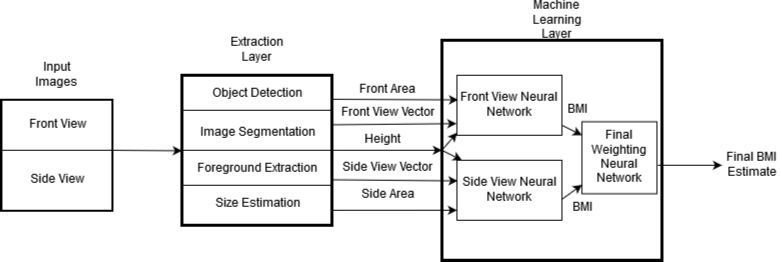
\includegraphics[width=\linewidth]{systemblock.png}
    \caption{System Block Diagram showing the processes input images undergo to estimate BMI.}
    \label{fig:systemblockdiagram}
\end{figure}

\begin{figure}[h]
    \centering
    \begin{minipage}[b]{0.3\textwidth}
    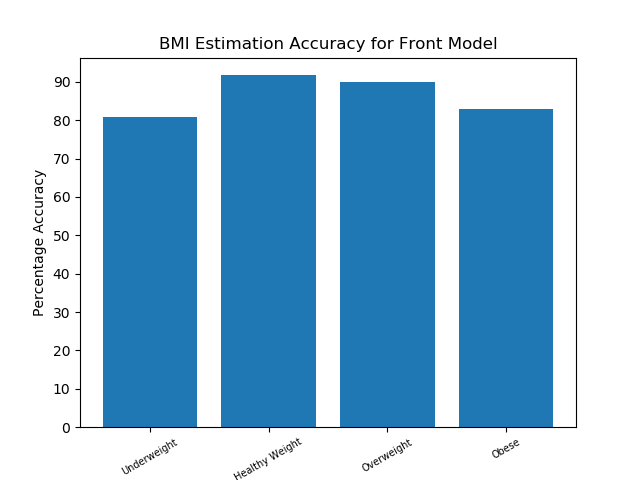
\includegraphics[width=\textwidth]{Front.png}
    \caption{Prediction Accuracy Across BMI Categories for Front Model.}
    \label{fig:frontaccuracy}
    \end{minipage}
    \hspace{1cm}
    \begin{minipage}[b]{0.3\textwidth}
    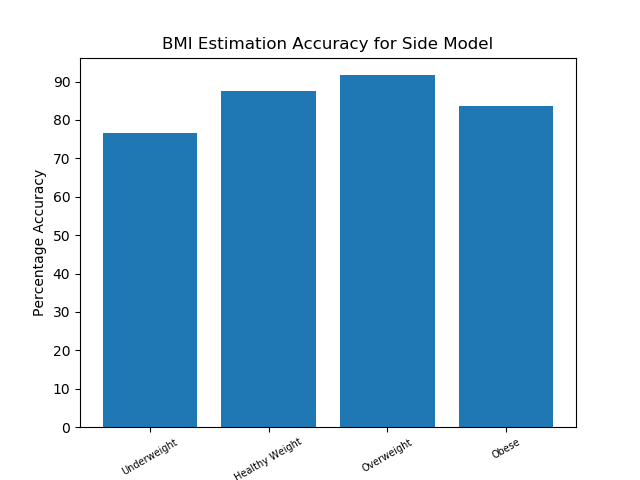
\includegraphics[width=\textwidth]{Side.png}
    \caption{Prediction Accuracy Across BMI Categories for Side Model.}
    \label{fig:sideaccuracy}
    \end{minipage}
\end{figure}

% \begin{figure}[h]
%     \centering
%     \begin{minipage}[b]{0.3\textwidth}
%     \includegraphics[width=\textwidth]{undererror.png}
%     \caption{Distribution of Percentage Error for BMI Estimations performed on the Underweight portion of the dataset.}
%     \label{fig:undererror}
%     \end{minipage}
%     \hspace{1cm}
%     \begin{minipage}[b]{0.3\textwidth}
%     \includegraphics[width=\textwidth]{healthyerror.png}
%     \caption{Distribution of Percentage Error for BMI Estimations performed on the Healthy portion of the dataset.}
%     \label{fig:healthyerror}
%     \end{minipage}
% \end{figure}

% \begin{figure}[h]
%     \centering
%     \begin{minipage}[b]{0.3\textwidth}
%     \includegraphics[width=\textwidth]{overerror.png}
%     \caption{Distribution of Percentage Error for BMI Estimations performed on the Overweight portion of the dataset.}
%     \label{fig:overerror}
%     \end{minipage}
%     \hspace{1cm}
%     \begin{minipage}[b]{0.3\textwidth}
%     \includegraphics[width=\textwidth]{obeseerror.png}
%     \caption{Distribution of Percentage Error for BMI Estimations performed on the Obese portion of the dataset.}
%     \label{fig:obeseerror}
%     \end{minipage}
% \end{figure}

% \begin{figure}[h]
%     \centering
%     \begin{minipage}[b]{0.3\textwidth}
%     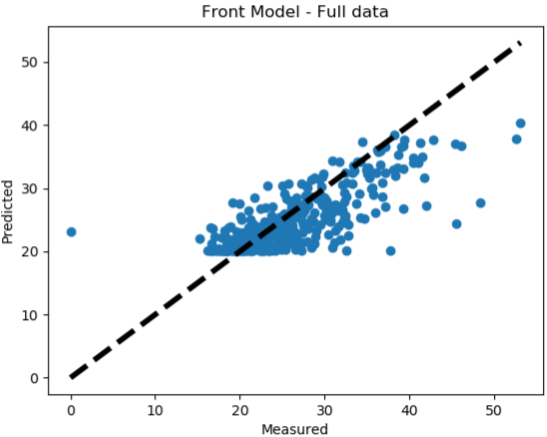
\includegraphics[width=\textwidth]{frontscatter.png}
%     \caption{Front Model Performance for Total dataset.}
%     \label{fig:frontscatter}
%     \end{minipage}
%     \hspace{1cm}
%     \begin{minipage}[b]{0.3\textwidth}
%     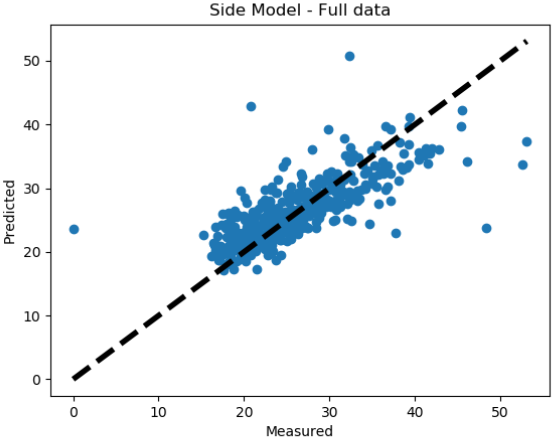
\includegraphics[width=\textwidth]{sidescatter.png}
%     \caption{Side Model Performance for Total dataset.}
%     \label{fig:sidescatter}
%     \end{minipage}
% \end{figure}
\end{document}

% budget
% system diagrams